\chapter{Uvod}
\label{ch:introduction_background}

\selectlanguage{croatian}

Otvoreni podaci postaju sve važniji resurs u modernom društvu, omogućavajući transparentnost, inovacije i društveni napredak. Međutim, sama dostupnost podataka ne jamči njihovu efektivnu iskoristivost. Iako standardizirani formati metapodataka poput DCAT-a~\cite{dcat2020} omogućavaju lakše otkrivanje i tumačenje pojedinačnih skupova podataka~\cite{janssen2012benefits}, dodatna vrijednost leži u njihovom povezivanju i otkrivanju novih uvida i skrivenog znanja~\cite{bizer2009linked}.

Nagli uspon alata umjetne inteligencije temeljenih na velikim jezičnim modelima~\cite{brown2020language,devlin2018bert} predstavlja obećavajući smjer za razvoj naprednih alata koji bi običnim korisnicima pružili nove mogućnosti korištenja otvorenih podataka. Ovi alati mogu automatizirati složene zadatke poput semantičkog pretraživanja, povezivanja skupova podataka i generiranja upita na prirodnom jeziku.

Ovaj rad fokusira se na razvoj sustava za analizu metapodataka otvorenih skupova podataka koji kombinira napredne tehnike umjetne inteligencije s tradicionalnim metodama obrade podataka. Glavni cilj je stvoriti alat koji omogućava korisnicima bez tehničke pozadine da učinkovito otkrivaju, analiziraju i povezuju skupove podataka kroz intuitivno sučelje na prirodnom jeziku.

Sustav je implementiran koristeći moderne tehnologije i pristupe uključujući RAG (Retrieval-Augmented Generation) arhitekturu~\cite{lewis2020retrieval}, vektorske baze podataka~\cite{wang2023vector} za semantičko pretraživanje i velike jezične modele za generiranje SPARQL upita. Ova kombinacija omogućava napredno razumijevanje korisničkih namjera i precizno otkrivanje relevantnih skupova podataka.

Evaluacija sustava provedena je na EU Portalu otvorenih podataka, jednom od najvećih izvora otvorenih podataka u Europi. Rezultati pokazuju značajna poboljšanja u usporedbi s tradicionalnim pristupima pretraživanja, posebno u području semantičkog razumijevanja i otkrivanja povezanih skupova podataka.

Rad je strukturiran u četiri glavna poglavlja koja pokrivaju uvod, dizajn i implementaciju sustava, evaluaciju rezultata i zaključak. Svako poglavlje fokusira se na specifične aspekte razvoja i evaluacije sustava, pružajući sveobuhvatan pregled cijelog projekta.

\begin{figure}[h!]
    \centering
    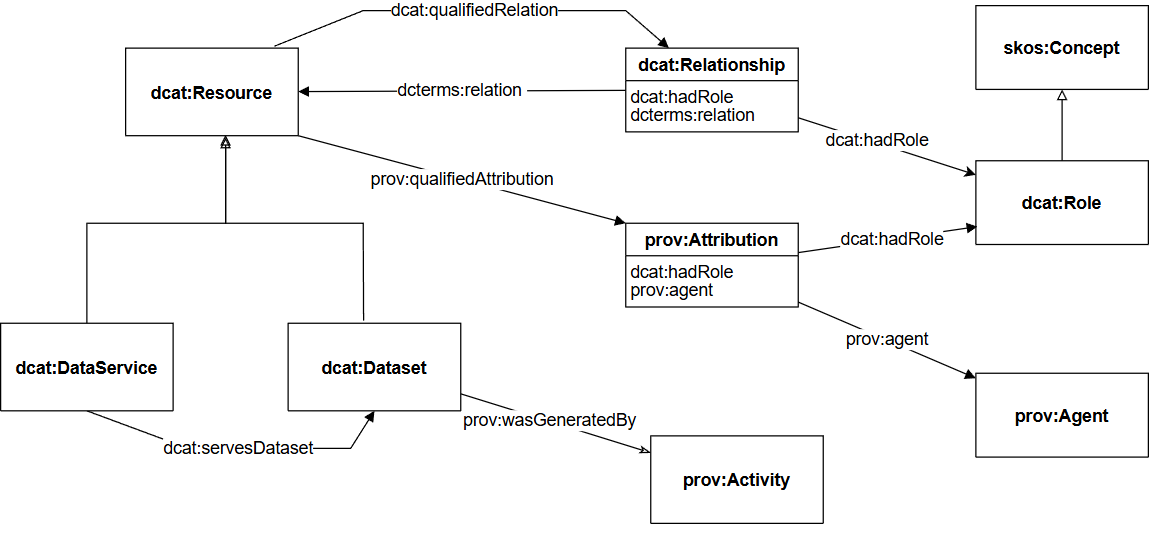
\includegraphics[width=1\textwidth]{figures/dcat.png}
    \caption{DCAT standard - prikazuje osnovne klase i svojstva metapodataka}
    \label{fig:dcat_standard}
\end{figure}